%%% FP2001.tex 05.10.2000 - Vesa Kolhinen <vesa.kolhinen@phys.jyu.fi>
%%% Original version:
%%% FP2000.tex 12.10.1999 - Eero Noponen <eero.noponen@hut.fi>
%%%
%%%
%%%
%%% Sample LaTeX file for the abstracts for the Proceedings of the
%%% Annual Meeting of the Finnish Physical Society.

\documentclass[12pt]{article}
\usepackage{fp2009}
\usepackage[T1]{fontenc}
\usepackage[latin1]{inputenc}
\usepackage{hyperref}

%%% Remove the following line if Times font is unavailable.
\usepackage{times}

%%% The following line is required if the document contains figures.
\usepackage{graphicx}

%%% The following line is for LaTeX 2.09.
%\documentstyle[FP2001,12pt]{article}

\begin{document}

%%%
%%% The title of the abstract is given here as \title{TITLE TEXT}.
%%%
\title{USING GIT DISTRIBUTED VERSION CONTROL TOOL TO MANAGE HEP DATA ANALYSIS PROJECT}
%\title{USING GIT DISTRIBUTED VERSION CONTROL TOOL TO MAINTAIN PHYSICS
%  CODE AND INTEROPERATE WITH CERN SUBVERSION REPOSITORIES}
%%%
%%% The list of authors; underline the name of the author who is responsible
%%% for the presentation of the paper.
%%%
\underline{P. Kaitaniemi}$^{1, 2}$ A. Heikkinen$^1$ 

%%%
%%% The address.
%%%
$^1$~P.O.Box 64 (Gustaf H\"allstr\"omin katu 2), FIN-00014 University of Helsinki, Finland\\
email: pekka.kaitaniemi@gmail.com

$^2$~CEN-Saclay, CEA-IRFU/SPhN, 91 191 Gif sur Yvette, France
%%% Do not remove.
\vspace{\baselineskip}
%%%
%%% Body text begins here.
%%%
% intro

Version control allows software developers to keep track of project history in
a systematic and detailed manner. 
%The project can be a data analysis or simulation program source code, 
%or even LaTeX code of a paper or thesis. 
In addition to tracking history, version control tools allow
one to merge contributions between several authors.
% background
Recently CERN has chosen to upgrade centralised CVS version control
system \cite{cernsvn} to another modernised centralised system called Subversion (SVN) \cite{svnsite}.
Unfortunately it does not offer the flexibility of the
distributed systems we are interested in. 

%%% The following minipage structures are needed to position the figure
%%% beside the text paragraph.
%%% For a standard figure environment, see the example below.

\begin{minipage}{6cm}
% git details
Git, a distributed version control tool \cite{torvalds}, however, 
provides this flexibility, 
and can be used as a ``super client'' with the CERN SVN service.
We discuss advantages of distributed version control tools,
such as Git, over traditional centralised ones. 
Most significant advantage is that the distributed
tools don't need a central server, and users can utilise
version control locally on their own computers without
heavy support infrastructure.
% our case and example image
We present an example use case for Git (Fig.~1), 
together with CERN central SVN version control for high energy physics data
analysis software maintenance~\cite{pk09aProceedings}.

\end{minipage}
 \hfill
 \begin{minipage}{8cm}
%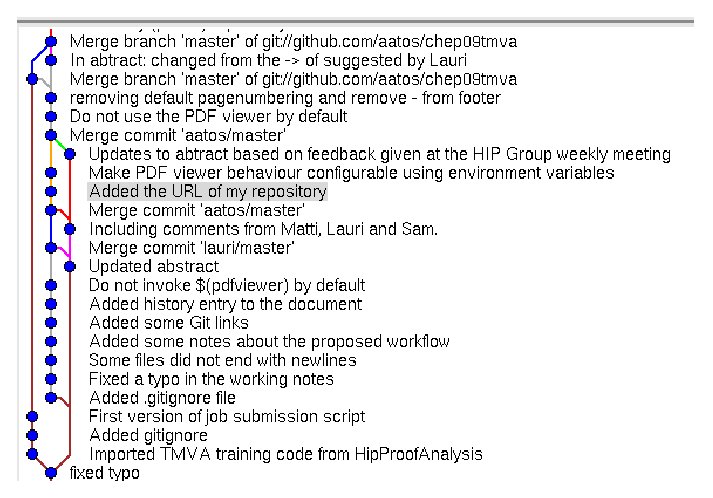
\includegraphics[width=12cm]{history.eps}
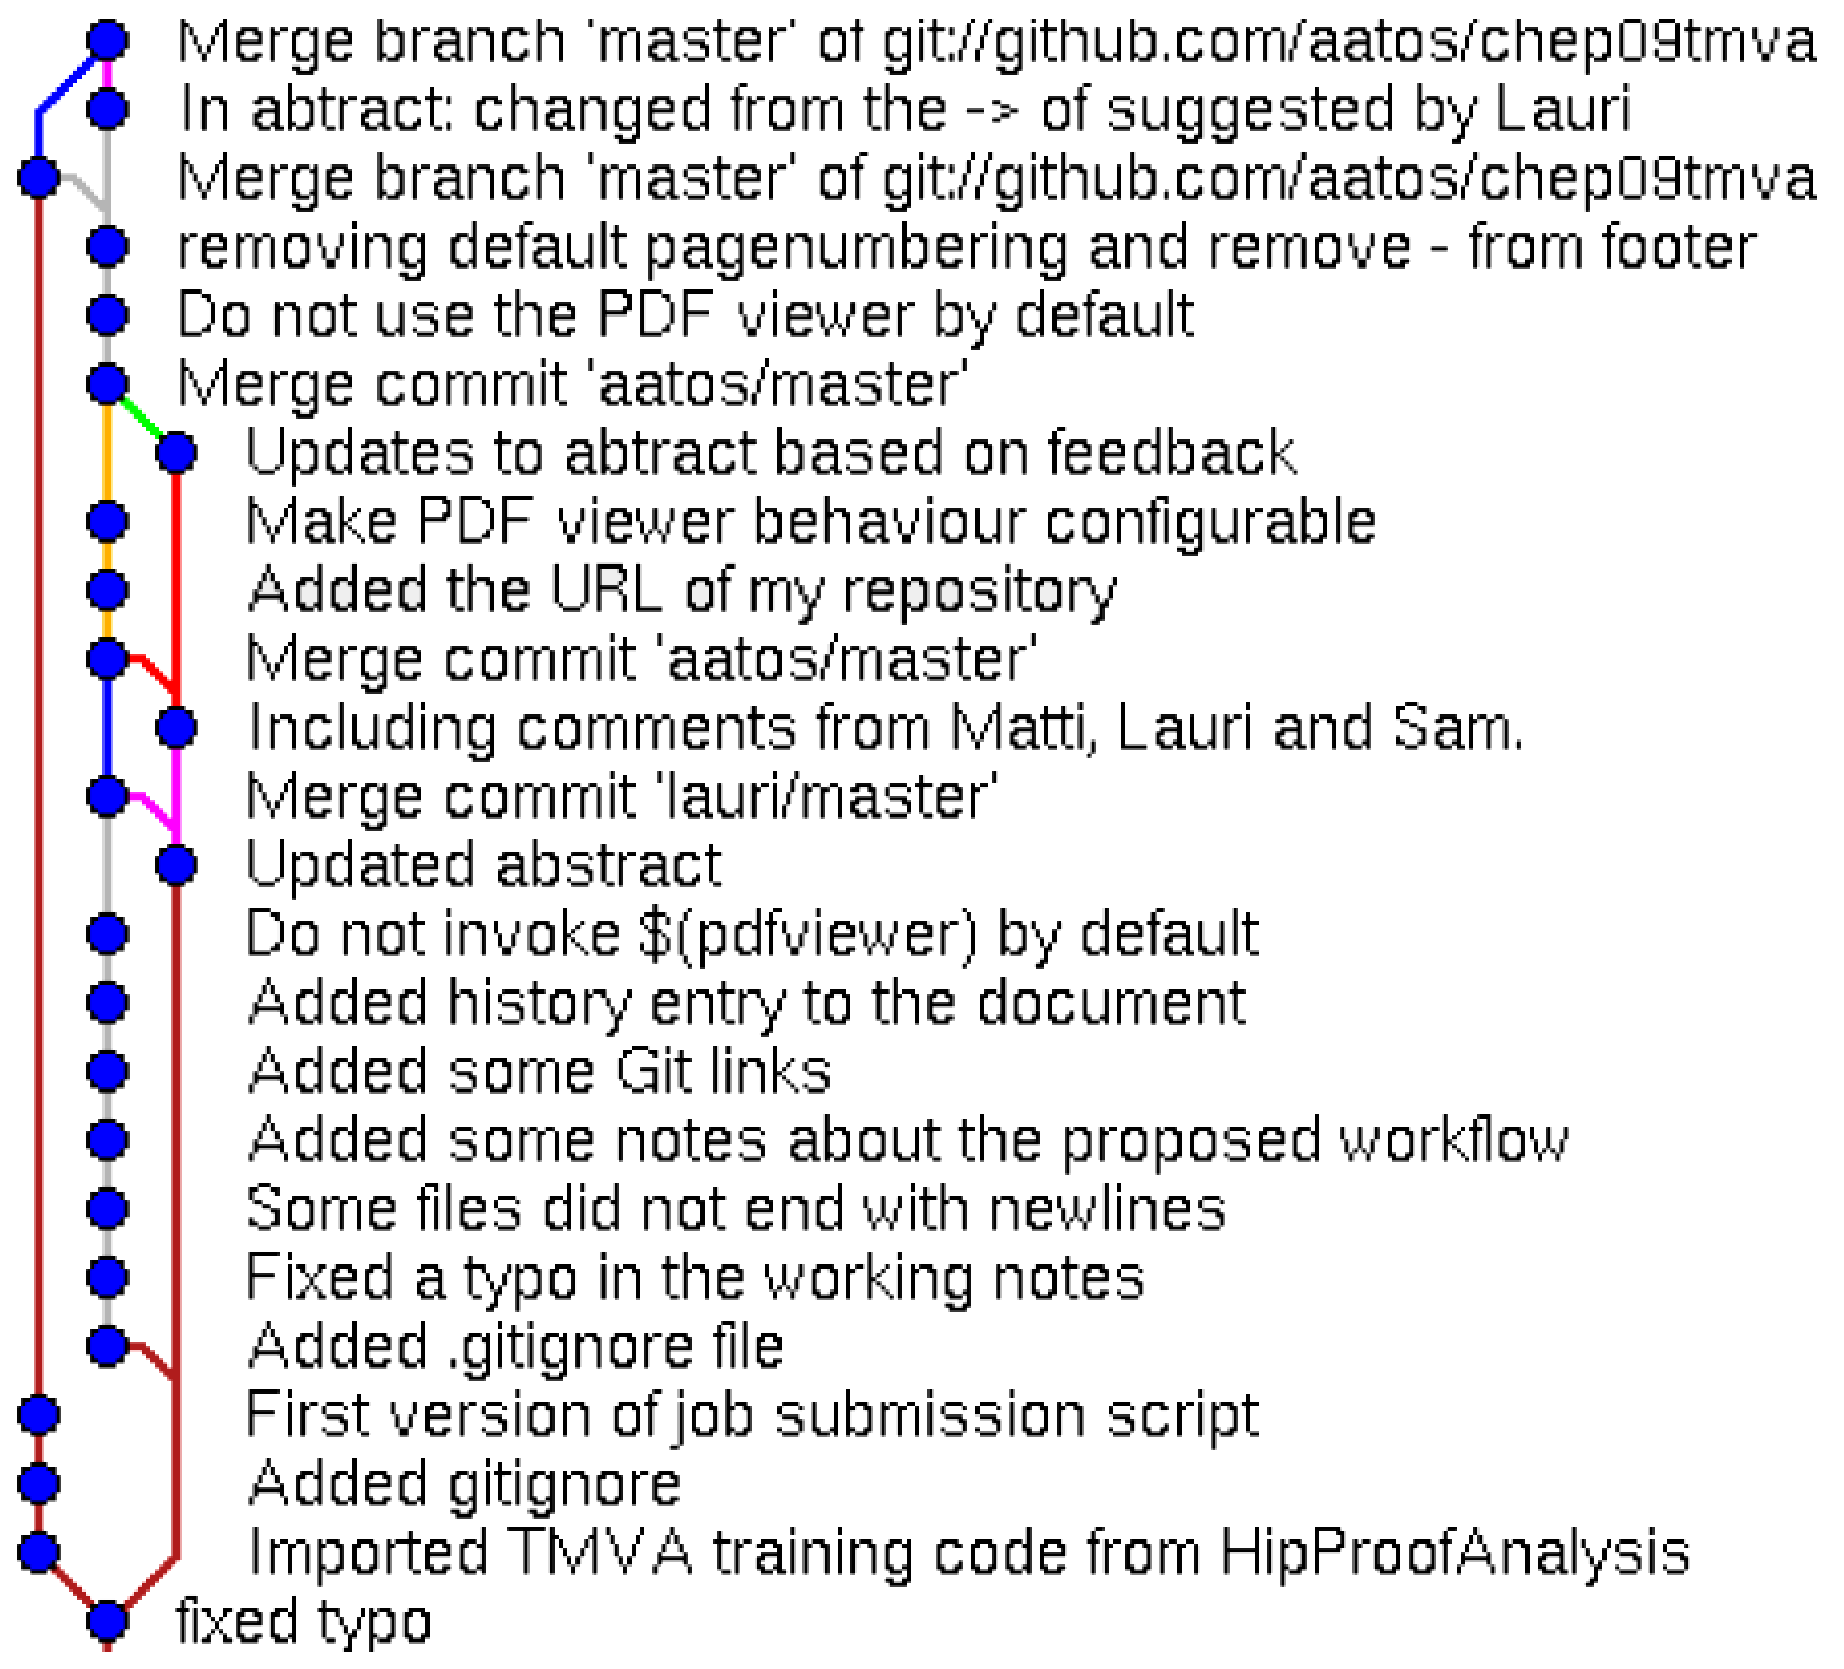
\includegraphics[width=8cm]{gitk.eps} 
{\bf Fig.1}:~Gitk tool showing branching and merging actions
performed during the development of the software.
\end{minipage}

%%%
%%% A more typical Figure.
%%%
%\begin{figure}[!h]
%\centering
\includegraphics[width=4cm]{logo.eps}
%\caption{Mallikuva.}
%\end{figure}

%%%
%%% The bibliography: the references are listed here.
%%%
\begin{thebibliography}{9}
\bibitem{cernsvn}
\href{http://cern.ch/svn}{CERN central SVN service (http://cern.ch/svn)}

\bibitem{svnsite}
\href{http://subversion.tigris.org}{Subversion website (http://subversion.tigris.org)}

\bibitem{torvalds}
L.Torvalds with the Linux kernel team,
Git Version Control System website,
\href{http://git-scm.com/}{http://git-scm.com/}

%\bibitem{gitsite} % same as \bibitemtorvalds
%\href{http://git.or.cz}{Git website (http://git.or.cz)}%

\bibitem{pk09aProceedings}
P.~Kaitaniemiemi and A.~Heikkinen et al.,
Ideal $\tau$-tagging with TMVA multivariate data-analysis toolkit,
Proceedings of International Conference on 
Computing in High Energy and Nuclear Physics, CHEP'09
(To be published)

\end{thebibliography}
\end{document}
